\documentclass{article} \usepackage{amsmath} \usepackage{amssymb} \usepackage{amsthm} \usepackage[margin=0.2in]{geometry} \usepackage{hyperref} \usepackage{physics} \usepackage{tikz} \usepackage{mathtools} \mathtoolsset{showonlyrefs} \theoremstyle{definition} \newtheorem{theorem}{Theorem}[section] \newtheorem{corollary}{Corollary}[theorem] \newtheorem{lemma}[theorem]{Lemma} \newtheorem{definition}{Definition}[section] \author{Connor Duncan} \date{\today}
\title{Physics-105-Lecture-Notes-02-05-2019}
\begin{document}
\maketitle\tableofcontents
\noindent\abstract{A single PDF with all lectures in a single document can be downloaded at \url{https://www.dropbox.com/sh/8sqzvxghvbjifco/AAC9LoSRnsRQDp7pYedgWpQMa?dl=0}. The password is 'analytic.mech.dsp'.
 This file was automatically generated using a script, so there might be some errors. If there are, you can contact me at \url{mailto:ctdunc@berkeley.edu}.}
\subsection{Examples of Lagrangian Mechanics} \subsubsection{Cone?} Missed the first one, but we know that \emph{angular momentum is conserved}. Basically, just a whole lot of algebran happening here, with something rotating in a conic shape, or on the surface of a cone (maybe like throwing a coin into one of those things at McDonalds). Stable solutions can be given by $\ddot r=0$. I.e. the coin doesn't ever go into the money receptacle. Gives that $\dot\theta^2\tan\alpha=\frac{g}{r_0}\Rightarrow\dot\theta^2=\frac{\omega_0}{\tan\alpha}$ Which implies that in order to have some stable orbit in a cone at a certain angle $\alpha$, you have explicit angular momentum dependence. \begin{center} 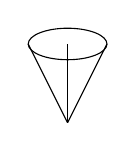
\begin{tikzpicture} \draw (0,1) ellipse (.5 and .2); \draw (0,0) -- (-.5,1); \draw (0,0)--(.5,1); \draw (0,0)--(0,1); \end{tikzpicture} \end{center} \subsubsection{Mass/Spring on a T} Imagine some $T$ on a tabletop, that looks a bit like this \begin{center} 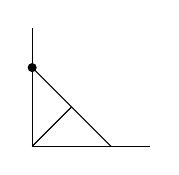
\begin{tikzpicture} \draw (0,0)--(1.5,0); \draw (0,0)--(0,1.5); \draw (0,0)--(.5,.5); \draw (1,0)--(0,1); \draw[fill] (0,1) ellipse (.05); \end{tikzpicture} \end{center} Where the dot is connected to the $T$ by a spring that's hooked up at the juncture. Let $\omega t$ be the angle between the x-axis and the $T$. then we can write $\vec{r}=(l\cos\omega t-\rho\sin\omega t)\hat x+(l\sin\omega t+\rho\cos\omega t)\hat y$ \begin{equation} T=\frac{1}{2}m(\dot r\dot r)=\frac{1}{2}m(\omega^2(l^2+\rho^2)+\dot\rho^2+2\omega l\dot\rho)\\ \end{equation} put in to the euler lagrange equation \begin{align} \pdv{L}{\rho}=m\omega^2\rho-k\rho\\ \pdv{L}{\dot\rho}=m\dot\rho+\omega l\\ \end{align} So, equating these two things, gives us that \begin{align} \ddot\rho+(\frac{k}{m}-\omega^2)\rho=0 \end{align} which yields 3 sort of `classes' of solutions. First is where $\omega<\sqrt{\frac{k}{m}}$, which yields a simple harmonic oscillator, very fun! We also could have $\omega>\sqrt{\frac{k}{m}}$, which gives us that $\rho(t)=Be^{\alpha t}+Ce^{-\alpha t}$. There's also the case of equality, which gives us resonant oscillation, or just a growth term $\rho(t)\sim t$. \subsubsection{Now with Gravity!} Take the previous problem, and just add gravity into the mix, since we all like to have fun. Now we have $V=mgy$, and we have $y$ from the previous problem, so the lagrangian becomes some really long wild thing, that I cannot see (Bale didn't do the whole thing out, but the principle of the problem is similar to what we did above). \section{Symmetries (Formally)} Considering changes to $L$ (the lagrangian) when we perturb one of the coordinates. Say it's $q_i\rightarrow \tilde q_i=q_i+k_i$ \subsection{Linear Momentum} consider \begin{align} \tilde x =x+\epsilon && \dot{\tilde x}=\dot x\\ T=\frac{1}{2}m\dot x^2=\frac{1}{2}m\dot{\tilde{x}^2}\\ L=\frac{1}{2}m\dot x^2-V(x) && \tilde L=\frac{1}{2}m\dot{\tilde{x}^2}-\tilde V(x) \end{align} If we apply the constraint that $L(x,\dot x)=\tilde L(\tilde x,\dot{\tilde x})$, then $V(x)$ has to be invariant to spatial pertubation, which implies that $F_x=0$, since $-F=\pdv{V}{x}$. This is just a meme'd way of writing conservation of linear momentum, since it boils down to \begin{equation} \dv{}{t} \left(m\dot x\right)=0 \end{equation} \subsection{Noethers Theorem (intro)} \begin{align} L(q,\dot q)=L(q+\epsilon k,\dot q+\epsilon\dot k)\\ L(q,\dot q)=L(q+\epsilon k,\dot q+\epsilon\dot k)=L(q,\dot q)+\epsilon\sum_i\dot k_i\pdv{L}{\dot q_i}+\epsilon\sum_ik\pdv{L}{q_i}....\\ \end{align} This just applies the constraint that the sum of the first n taylor expanded terms has to be zero, which is \emph{Noethers Theorem}. Another, simpler way of writing this is that \begin{equation} \sum K\pdv{L}{\dot q}=C \end{equation} where $C$ is constant. \paragraph{Example} \begin{center} 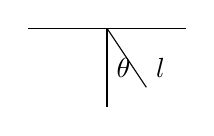
\begin{tikzpicture} \draw (-1,1)--(1,1); \draw (0,1)--(0.5,0.25); \draw (0,.5) node[anchor=west]{$\theta$}; \draw (.5,.5) node[anchor=west]{$l$}; \draw (0,0)--(0,1); \end{tikzpicture} \end{center} we just apply \begin{equation} L=\frac{1}{2}m\dot l^2+\frac{1}{2}ml^2\dot\theta^2-mgl\cos\theta \end{equation} And derive properties from this, like conservation of angular momentum. \subsection{Probably the Hamiltonian} consider \begin{align} H=\dot q\pdv{L}{\dot q}-L\\ \dv{H}{t}=-\frac{dL}{dt} \end{align} some long thing using the chain rule. has it simplify down to the above form, which implies htat $H$ is a conserved quantity with respect to time. Take \begin{align} L=\frac{1}{2}m\dot x^2-V(x)\\ H=\dot x\frac{dL}{d\dot x}-L=m\dot x^2-(\frac{1}{2}m\dot x^2+V(x))=\text{total energy} \end{align} which lets us say $H$ is a total energy, the \emph{hamiltonian}.
\end{document}
